\documentclass{beamer}
\usepackage[utf8]{inputenc}
\usepackage{graphicx}
\usepackage{subfig}
\author[Sowmya Vajjala]{Instructor: Sowmya Vajjala}


\title[LING 120]{LING 120, Fall 2017 \\ Language and Computers}

\date{29 September 2017}

\institute{Iowa State University, USA}

%%%%%%%%%%%%%%%%%%%%%%%%%%%

\begin{document}

\begin{frame}\titlepage
\end{frame}

\begin{frame}
\frametitle{Class outline}%5minutes
\begin{enumerate}
\item Continuing from where we left
\item Review of Topic 4 (by asking more questions!)
\item Time to choose mid-term topics for teams
\end{enumerate}
\end{frame} %\item Assignment 3 Description - do this on Monday

\begin{frame}[fragile]
\frametitle{Grep and Egrep - tools to search large files/folders using regular expressions}
\begin{itemize}
\item Available by default on Unix based operating systems (Mac, Ubuntu etc)
\item Windows 10 perhaps supports it (I don't know - you should tell me!) \pause
\item Brief demo of using egrep:
\begin{verbatim}
egrep 'Stockmann' pg2446.txt
egrep '[[:digit:]]' pg2446.txt
egrep 'Petra|Horster' pg2446.txt
egrep 'Petra|Horster' pg2446.txt | wc
egrep 'th(e|i)s' pg2446.txt
egrep 'th(e|i)s*' pg2446.txt
\end{verbatim}
\end{itemize}
\end{frame}

\begin{frame}
\frametitle{Regular Expressions: Practice}
Work in groups of 3 people, download pg2446.txt from \url{https://goo.gl/gSnhGD}, and answer the following questions using regular expressions.
\begin{itemize}
\item Whose name occurs more at the beginning of a line - Dr Stockmann or Mrs Stockmann? How many times?
\item What is the difference between \textit{egrep 't.s' pg2446.txt} and \textit{egrep 't.*s' pg2446.txt}?
\item In general, what will the pattern \textit{joh?n} identify? How will you verify?
\item What will \textit{egrep -o 'Stockmann' pg2446.txt} do? Why? What happens if you remove the -o?
\item How many times do Stockmann and Petra appear in the same line in this file?
\end{itemize}
Note: Regular expressions cheatsheets, egrep help can be found by searching online. 
\end{frame}

%Review of search
\begin{frame}
\frametitle{Review: Precision and Recall}
\framesubtitle{source: Wikipedia page on the topic: \url{https://goo.gl/4gdNRd}}
\begin{center}
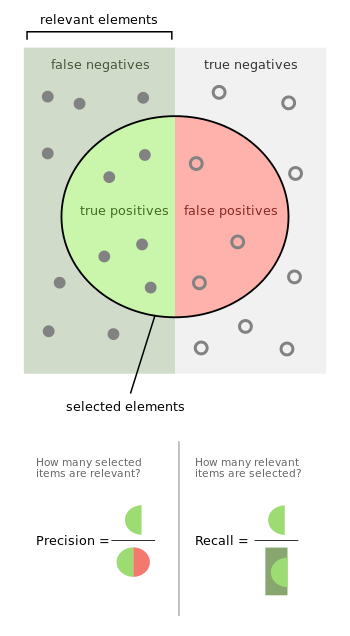
\includegraphics[width=0.4\textwidth]{Precisionrecall.png}
\end{center}
\end{frame}

\begin{frame}
\frametitle{Review: Precision and Recall}
\framesubtitle{source: questions obtained from textbook and quora.com}
\begin{minipage}{0.3\textwidth}
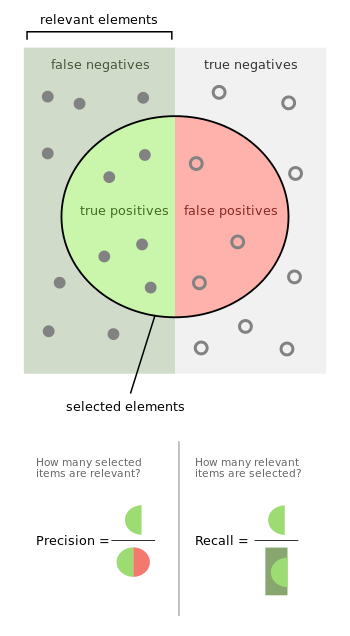
\includegraphics[width=\linewidth]{Precisionrecall.png}
\end{minipage}%
\begin{minipage}{0.6\textwidth}
What is important in the following cases - precision or recall?
\begin{itemize}
\item Identifying cases where a cancer curing drug has a side effect of nausea \pause
\item Identifying cases where a cancer curing drug has a side effect of death \pause
\item Let us say there is a Zombie apocalypse and you are building a safe zone for the non-Zombies. What is a high recall scenario here? What is desirable?
\end{itemize}
\end{minipage} \bigskip
\end{frame}
%Discussion questions: 5, 8, 10 in the textbook for Chapter 4.

\begin{frame}
\frametitle{How structured/unstructured is a google search?}
\begin{itemize}
\item What does: "What does a * do" show me on google? \pause
\item More tips from google on doing such searches:
\begin{itemize}
\item \url{https://support.google.com/websearch/answer/2466433?hl=en}
\item \url{https://support.google.com/vault/answer/2474474?hl=en}
\end{itemize}
\item \url{https://www.google.com/advanced_search?hl=en&fg=1} \pause
\item Why google does not support a full fledged regular expression search \\ - \url{https://www.youtube.com/watch?v=lYiTIDgejas} \pause
\item There used to be a Code Search platform by Google which indexed publicly accessible software code - that allowed regular expression search. 
\end{itemize}
\end{frame}

\begin{frame}
\frametitle{Quick recap of topics}
\begin{itemize}
\item Difference between structured and unstructured search
\item How does web-search work?
\item How can we use regular expressions to look for patterns? \pause
\item How is this knowledge useful?: You should now know how the knowledge of patterns and conventions in human language (English) are useful in information extraction. \pause
\item If that kind of stuff fascinated you, look for advanced courses on information retrieval, language processing etc (They will ultimately require you to learn to write computer programs!) \pause
\item Professional world: Software engineers, Search Engine Optimizers (yes, that is a title!), Search/Ad relevance evaluators, etc.
\end{itemize}
\end{frame}

%Exercise for today.
\begin{frame}
\frametitle{Today's attendance exercise}
\begin{itemize}
\item Group according to your mid-term teams.
\item Look at the list of topics and choose one for your team after discussion.
\item Start thinking about how to distribute work, what to present etc.
\item Return your topic choice along with team member names to me - that is your attendance for today. 
\item People who are absent today will just not participate in choosing. Don't worry about that.
\end{itemize}
\end{frame}

\begin{frame}
\frametitle{Next Week}
\begin{itemize}
\item Introduction to Natural Language Processing - language related issues that trouble a computer
\item No assigned readings!
\item Start working on Assignment 3
\item Start thinking about your mid-term presentation
\end{itemize}
\end{frame}

\end{document}
